\section{System Model}
\begin{frame}
  \frametitle{Multicell}
  \begin{figure}
    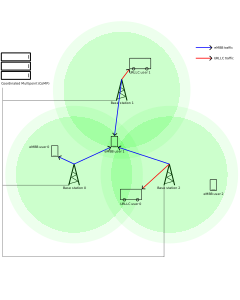
\includegraphics[width=0.5\textwidth]{model_multicell}
    \caption{Multicell model}
  \end{figure}
\end{frame}

\begin{frame}
  \begin{figure}
    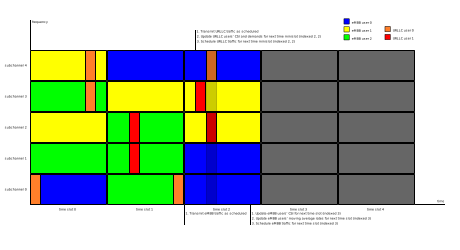
\includegraphics[width=1.05\textwidth]{framework_singlecell}
    \caption{Singlecell framework}
  \end{figure}
\end{frame}

\begin{frame}
  \frametitle{Stochastic Problem}
  \small
  \begin{maxi!}
    {\embbRaVec, \urllcRaVec, \urllcLaVec}{\sum_{\embbUser}{\utilityCompositeFunction{\embbAverageRateRandOne}}\label{pb:problem0}}
    {}{}
    \addConstraint
      {\sum_{\embbUser}{\embbRaFour}}
      {\leq 1\label{pb:problem1}}
      {\forall\timeSlot \forall\baseStation \forall\subchannel}
    \addConstraint
      {\embbRaFour}
      {\in \setDst{0, 1}\label{pb:problem2}}
      {\forall\embbUser \forall\timeSlot \forall\baseStation \forall\subchannel}
    \addConstraint
      {\sum_{\baseStation}{\urllcLaFour}}
      {\leq 1\label{pb:problem3}}
      {\forall\urllcUser \forall\timeSlot \forall\timeMinislot}
    \addConstraint
      {\urllcRaSix}
      {\leq \urllcLaFour\label{pb:problem4}}
      {\forall\urllcUser \forall\embbUser \forall\timeSlot \forall\timeMinislot \forall\baseStation \forall\subchannel}
    \addConstraint
      {\urllcLaFour}
      {\in \setDst{0, 1}\label{pb:problem5}}
      {\forall\urllcUser \forall\timeSlot \forall\timeMinislot \forall\baseStation}
    \addConstraint
      {\sum_{\urllcUser}{\urllcRaSix}}
      {\leq \embbRaFour\label{pb:problem6}}
      {\forall\embbUser \forall\timeSlot \forall\timeMinislot \forall\baseStation \forall\subchannel}
    \addConstraint
      {\urllcRateRandThree}
      {\geq \demandRandThree\label{pb:problem7}}
      {\forall\urllcUser \forall\timeSlot \forall\timeMinislot}
    \addConstraint
      {\urllcRaSix}
      {\in \setDst{0, 1}\label{pb:problem8}}
      {\forall\urllcUser \forall\embbUser \forall\timeSlot \forall\timeMinislot \forall\baseStation \forall\subchannel}
  \end{maxi!}
\end{frame}

\begin{frame}
  \begin{itemize}
    \item The system maximizes eMBB traffic's total average rate and fairness \eqref{pb:problem0}.
    \item For each time slot, the system
      \begin{itemize}
        \item allocates a subchannel to at most one eMBB user \eqref{pb:problem1}.
        \item either un-allocates or allocates a subchannel to an eMBB user \eqref{pb:problem2}.
      \end{itemize}
  \end{itemize}
\end{frame}

\begin{frame}
  \begin{itemize}
    \item For each time minislot, the system
      \begin{itemize}
        \item associates at most one base station to a URLLC user \eqref{pb:problem3}.
        \item allocates a subchannel to a URLLC user only if it associates the corresponding base station to the user \eqref{pb:problem4}.
        \item either un-associates or associates a base station to a URLLC user \eqref{pb:problem5}.
        \item allocates a subchannel to at most one URLLC user, and punctures the subchannel for a URLLC user only if it allocates the subchannel to the corresponding eMBB user \eqref{pb:problem6}\proofFootnote.
        \item serves demands of URLLC users without delays \eqref{pb:problem7}.
        \item employs URLLC puncturing scheme instead of superposition \eqref{pb:problem8}.
      \end{itemize}
  \end{itemize}
\end{frame}

\subsection{eMBB Problem}
\begin{frame}
  \frametitle{eMBB Problem}
  \begin{maxi!}
    {\embbRaVec}{\sum_{\embbUser}{\utilityCompositeFunction{\embbAverageRateRandOne}}}
    {}{}
    \addConstraint
      {\sum_{\embbUser}{\embbRaFour}}
      {\leq 1}
      {\forall\timeSlot \forall\baseStation \forall\subchannel}
    \addConstraint
      {\embbRaFour}
      {\in \setDst{0, 1}}
      {\forall\embbUser \forall\timeSlot \forall\baseStation \forall\subchannel}
  \end{maxi!}
\end{frame}

\begin{frame}
  \frametitle{Relaxed eMBB Problem}
  \begin{maxi!}
    {\embbRaVecRelax}{\sum_{\embbUser}{\utilityCompositeFunction{\embbAverageRateRandOneRelax}}}
    {}{}
    \addConstraint
      {\sum_{\embbUser}{\embbRaFourRelax}}
      {\leq 1}
      {\forall\timeSlot \forall\baseStation \forall\subchannel}
    \addConstraint
      {\embbRaFourRelax}
      {\geq 0}
      {\forall\embbUser \forall\timeSlot \forall\baseStation \forall\subchannel}
  \end{maxi!}
\end{frame}

\begin{frame}
  \frametitle{Gradient Problem}
  \begin{maxi!}
    {\embbRaVecOneRelaxCur}{\sum_{\embbUser}{\frac{\embbRateTwoRelaxCur}{\embbMovingAverageRateTwoRelaxCur}}}
    {}{}
    \addConstraint
      {\sum_{\embbUser}{\embbRaFourRelaxCur}}
      {\leq 1}
      {\forall\baseStation \forall\subchannel}
    \addConstraint
      {\embbRaFourRelaxCur}
      {\geq 0}
      {\forall\embbUser \forall\baseStation \forall\subchannel}
  \end{maxi!}
\end{frame}

\begin{frame}
  \begin{itemize}
    \item The relaxed moving average rate of eMBB user is defined based on exponential moving average (EMA) as
      \begin{equation}
        \forall\embbUser \colon \embbMovingAverageRateTwoRelax =
          \begin{cases}
            \frac{1}{\timeSlotsNum} \sum_{\baseStation, \subchannel}{\frac{1}{\embbUsersNum} \embbPeakRateFour} &\timeSlot = 0\\
            \left(1 - \smoothingFactor\right) \embbMovingAverageRateTwoRelaxDecrement + \smoothingFactor \embbRateTwoRelaxDecrement &\nonzeroTimeSlots
          \end{cases} \bpsl.
      \end{equation}
  \end{itemize}
\end{frame}

\begin{frame}
  \begin{itemize}
    \item The initial value of which is defined by the feasible policy $\embbRaVecRelaxCandidate$ for the relaxed eMBB problem where\proofFootnote
      \begin{equation}
        \embbMovingAverageRateInitialValuePolicy.
      \end{equation}
  \end{itemize}
\end{frame}

\begin{frame}
  \begin{itemize}
    \item Given a policy $\embbRaVecCandidate$ where for $\timeSlot = 0, \dots, \timeSlotsNum - 1$, $\embbRaVecOneCandidate$ is a basic optimal point for the $\timeSlot^{th}$ gradient problem, then $\embbRaVecCandidate$ is an asymptotically optimal policy for the eMBB problem\proofFootnote.
  \end{itemize}
\end{frame}

\begin{frame}
  \begin{itemize}
    \item However, simplex methods run in exponential time in worst-case scenarios.
  \end{itemize}
\end{frame}

\begin{frame}
  \begin{itemize}
    \item The following policy is asymptotically optimal with respect to the eMBB problem\proofFootnote:
      \begin{equation}
        \forall\timeSlot \colon \embbPolicy.
      \end{equation}
  \end{itemize}
\end{frame}

\subsection{URLLC Problem}
\begin{frame}
  \frametitle{URLLC Problem}
  \small
  \begin{maxi!}
    {\urllcRaVecOneSlotCur, \urllcLaVecOneSlotCur}{\sum_{\embbUser}{\frac{\embbRateTwoRelaxCur}{\embbMovingAverageRateTwoRelaxCur}}}
    {}{}
    \addConstraint
      {\sum_{\baseStation}{\urllcLaFourSlotCur}}
      {\leq 1}
      {\forall\urllcUser \forall\timeMinislot}
    \addConstraint
      {\urllcRaSixSlotCur}
      {\leq \urllcLaFourSlotCur}
      {\forall\urllcUser \forall\embbUser \forall\timeMinislot \forall\baseStation \forall\subchannel}
    \addConstraint
      {\urllcLaFourSlotCur}
      {\in \setDst{0, 1}}
      {\forall\urllcUser \forall\timeMinislot \forall\baseStation}
    \addConstraint
      {\sum_{\urllcUser}{\urllcRaSixSlotCur}}
      {\leq \embbRaFourCandidateCur}
      {\forall\embbUser \forall\timeMinislot \forall\baseStation \forall\subchannel}
    \addConstraint
      {\urllcRateRandThreeSlotCur}
      {\geq \demandRandThreeSlotCur}
      {\forall\urllcUser \forall\timeMinislot}
    \addConstraint
      {\urllcRaSixSlotCur}
      {\in \setDst{0, 1}}
      {\forall\urllcUser \forall\embbUser \forall\timeMinislot \forall\baseStation \forall\subchannel}
  \end{maxi!}
\end{frame}

\begin{frame}
  \frametitle{Puncturing Problem}
  \begin{mini!}
    {\urllcRaVecTwoCur, \urllcLaVecTwoCur}{\sum_{\urllcUser, \embbUser, \baseStation, \subchannel}{\frac{\embbPeakRateFourCur}{\embbMovingAverageRateTwoRelaxCur} \urllcRaSixCur}}
    {}{}
    \addConstraint
      {\sum_{\baseStation}{\urllcLaFourCur}}
      {\leq 1}
      {\forall\urllcUser}
    \addConstraint
      {\urllcRaSixCur}
      {\leq \urllcLaFourCur}
      {\forall\urllcUser \forall\embbUser \forall\baseStation \forall\subchannel}
    \addConstraint
      {\urllcLaFourCur}
      {\in \setDst{0, 1}}
      {\forall\urllcUser \forall\baseStation}
    \addConstraint
      {\sum_{\urllcUser}{\urllcRaSixCur}}
      {\leq \embbRaFourCandidateCur}
      {\forall\embbUser \forall\baseStation \forall\subchannel}
    \addConstraint
      {\urllcRateThreeCur}
      {\geq \demandThreeCur}
      {\forall\urllcUser}
    \addConstraint
      {\urllcRaSixCur}
      {\in \setDst{0, 1}}
      {\forall\urllcUser \forall\embbUser \forall\baseStation \forall\subchannel}
  \end{mini!}
\end{frame}

\begin{frame}
  \begin{itemize}
    \item Given a time slot policy $\tuple{\urllcRaVecOneCandidateSlotCur, \urllcLaVecOneCandidateSlotCur}$ where for $\timeMinislot = 0, \dots, \timeMinislotsNum - 1$, $\tuple{\urllcRaVecTwoCandidateSlotCur, \urllcLaVecTwoCandidateSlotCur}$ solves the $\timeMinislot^{th}$ puncturing problem, then $\tuple{\urllcRaVecOneCandidateSlotCur, \urllcLaVecOneCandidateSlotCur}$ is an optimal point for the URLLC problem\proofFootnote.
  \end{itemize}
\end{frame}

\begin{frame}
  \frametitle{Scheduling Problem}
  \begin{mini!}
    {\urllcNpRaVecTwoCur, \urllcLaVecTwoCur}{\sum_{\urllcUser, \baseStation, \subchannel}{\costThreeCur \urllcNpRaFiveCur}}
    {}{}
    \addConstraint
      {\sum_{\baseStation}{\urllcLaFourCur}}
      {\leq 1}
      {\forall\urllcUser}
    \addConstraint
      {\urllcNpRaFiveCur}
      {\leq \urllcLaFourCur}
      {\forall\urllcUser \forall\baseStation \forall\subchannel}
    \addConstraint
      {\urllcLaFourCur}
      {\in \setDst{0, 1}}
      {\forall\urllcUser \forall\baseStation}
    \addConstraint
      {\sum_{\urllcUser}{\urllcNpRaFiveCur}}
      {\leq 1}
      {\forall\baseStation \forall\subchannel}
    \addConstraint
      {\sum_{\baseStation, \subchannel}{\urllcNpRaFiveCur \urllcPeakRateFourCur}}
      {\geq \demandThreeCur}
      {\forall\urllcUser}
    \addConstraint
      {\urllcNpRaFiveCur}
      {\in \setDst{0, 1}}
      {\forall\urllcUser \forall\baseStation \forall\subchannel}
  \end{mini!}
\end{frame}

\begin{frame}
  \begin{itemize}
    \item The puncturing cost of subchannel is defined as
      \begin{equation}
        \forall\timeSlot \colon \forall\baseStation \colon \forall\subchannel \colon \costThree = \max_{\embbUser}{\frac{\embbPeakRateFour}{\embbMovingAverageRateTwoRelax}}.
      \end{equation}
  \end{itemize}
\end{frame}

\begin{frame}
  \begin{itemize}
    \item The scheduling problem is equivalent to the puncturing problem\proofFootnote.
  \end{itemize}
\end{frame}

\begin{frame}
  \begin{itemize}
    \item The scheduling problem is independent from $\embbRaVec$.
  \end{itemize}
\end{frame}

\begin{frame}
  \frametitle{Homogeneous Problem}
  \begin{mini!}
    {\urllcNpRaVecTwoCur, \urllcLaVecTwoCur}{\minCostOneCur \sum_{\urllcUser, \baseStation, \subchannel}{\urllcNpRaFiveCur}}
    {}{}
    \addConstraint
      {\sum_{\baseStation}{\urllcLaFourCur}}
      {\leq 1}
      {\forall\urllcUser}
    \addConstraint
      {\urllcNpRaFiveCur}
      {\leq \urllcLaFourCur}
      {\forall\urllcUser \forall\baseStation \forall\subchannel}
    \addConstraint
      {\urllcLaFourCur}
      {\in \setDst{0, 1}}
      {\forall\urllcUser \forall\baseStation}
    \addConstraint
      {\sum_{\urllcUser}{\urllcNpRaFiveCur}}
      {\leq 1}
      {\forall\baseStation \forall\subchannel}
    \addConstraint
      {\sum_{\baseStation, \subchannel}{\urllcNpRaFiveCur}}
      {\geq \frac{\demandThreeCur}{\urllcMaxRateThreeCur}}
      {\forall\urllcUser}
    \addConstraint
      {\urllcNpRaFiveCur}
      {\in \setDst{0, 1}}
      {\forall\urllcUser \forall\baseStation \forall\subchannel}
  \end{mini!}
\end{frame}

\begin{frame}
  \begin{itemize}
    \item The minimum puncturing cost is defined as
      \begin{equation}
        \forall\timeSlot \colon \minCostOne = \min_{\baseStation, \subchannel}{\costThree}.
      \end{equation}
    \item The maximum rate of URLLC user is defined as
      \begin{equation}
        \forall\timeSlot \colon \forall\timeMinislot \colon \forall\urllcUser \colon \urllcMaxRateThree = \max_{\baseStation}{\urllcPeakRateFour}.
      \end{equation}
  \end{itemize}
\end{frame}

\begin{frame}
  \begin{itemize}
    \item $\minCostOneCur \sum_{\urllcUser}{\ceil{\frac{\demandThreeCur}{\urllcMaxRateThreeCur}}}$ is the optimal value for the homogeneous problem.
  \end{itemize}
\end{frame}

\begin{frame}
  \begin{itemize}
    \item The nearest association algorithm defines the following point:
      \begin{align*}
        \nearestAssociation.
      \end{align*}
  \end{itemize}
\end{frame}

\begin{frame}
  \begin{itemize}
    \item The nearest association algorithm is a $\frac{\maxCostOneCur}{\minCostOneCur}$-approximation algorithm for the scheduling problem\proofFootnote.
  \end{itemize}
\end{frame}

\begin{frame}
  \begin{itemize}
    \item The maximum puncturing cost is defined as
      \begin{equation}
        \forall\timeSlot \colon \maxCostOne = \max_{\baseStation, \subchannel}{\costThree}.
      \end{equation}
  \end{itemize}
\end{frame}

\begin{frame}
  \begin{itemize}
    \item The opportunistic nearest association algorithm defines the following point:
      \footnotesize
      \begin{align*}
        \forall\urllcUser \colon \urllcLaFourCandidateCur &=
          \begin{cases}
            1 &\baseStation = \min_{\baseStationCandidate}{\argmax_{\baseStationCandidate}{\urllcPeakRateFourCurBaseStationCandidate}}\\
            0 &\text{otherwise}
          \end{cases},\\
        \forall\baseStation \colon \forall\urllcUser \colon \urllcNpRaFiveCandidateCur &=
          \begin{cases}
            1 &
              \begin{aligned}
                &\left(\sum_{\urllcUserCandidate = 0}^{\urllcUser - 1}{\ceil{\frac{\demandThreeUserCandidateCur}{\urllcMaxRateThreeUserCandidateCur}} \urllcLaFourCandidateUserCandidateCur}\right) + 1\\
                \leq &\card{\left\{\subchannelCandidate \subjectTo \costThreeCur > \costThreeCurSubchannelCandidate \lor (\costThreeCur = \costThreeCurSubchannelCandidate \land \subchannel > \subchannelCandidate)\right\}}\\
                \leq &\sum_{\urllcUserCandidate = 0}^{\urllcUser}{\ceil{\frac{\demandThreeUserCandidateCur}{\urllcMaxRateThreeUserCandidateCur}} \urllcLaFourCandidateUserCandidateCur}
              \end{aligned}\\
            0 &\text{otherwise}
          \end{cases}.
      \end{align*}
  \end{itemize}
\end{frame}

\begin{frame}
  \begin{itemize}
    \item The opportunistic nearest association algorithm is an optimal algorithm for the scheduling problem in single-cell networks\proofFootnote.
  \end{itemize}
\end{frame}
